\section{Example of a 3-Way Join with Aggregation}
By performing a 3-Way join alongside aggregation, the correlation between CSC1015F course grades and Sakai usage is tested by working out the change of each student's class rank according to each of the benchmarks compared to their CSC1015F grade class ranking. Each benchmark/grade ranking change is then compared to Sakai usage. To achieve this, for each benchmarking dataset a derived dataset is created that contains numerical values of changes in class rank. Correlation between these datasets and Sakai usage is tested by finding correlation coefficients for each derived classRankChange dataset compared to the Sakai usage dataset. For this project, Sakai usage is proxied in terms of the number of times a student logs into the system - the rationale being that the more often students log into Sakai, the more they are using it.

\subsection{ETL}
Using nETL, rows are extracted from the three CSV files (\textit{Admissions (2014 - 2016).csv}, \textit{Grades (2014 - 2016).csv} and \textit{Events (2016).csv}) concurrently and independently of each other, in batches of 5 000, 10 000 and 30 000 rows, respectively.

By using nETL configuration, rows from the admissions data are selected for students who are South African citizens or permanents residents, and who are undergraduates; rows from the grades data are selected for undergraduate students who attended CSC1015F during 2016; rows from the events data are selected for presence events only. Dynamic filters are configured for the admissions and events data to only include students who took the CSC1015F course.

The events data contains a field \textit{ref}, which is a long string and is not required in the analysis. As such, this string is dropped through a whitelisting process prior to serialization and by loading strings into CouchDB (in batches via the \textit{\_bulk\_docs} endpoint). An example of a row from the event data serialized to a JSON string is shown in Figure \ref{fig-json-event}.

\begin{figure}[H]
    \centering
    \begin{mdframed}
        \centering
        \begin{minted}{text}
{
    "_id": "000e569ee321b915bae59fe62e0051e3",
    "_rev": "1-7112afce121087818c33ebfd0fd7fed7",
    "event_date": "2016-04-17T14:04:20.000Z",
    "event_id": 281, // anonymized student number
    "uct_id": 3018438,
    "site_key": 2297,
    "type_": "event"
}           
        \end{minted}
    \end{mdframed}
    \caption[Serialized events document]{\textbf{Figure \ref{fig-json-event}: Serialized events document}}
    \label{fig-json-event}
\end{figure}

\subsection{Indexing}
Since a single student may be associated with many rows in the events data (sometimes even thousands of rows), a reduce function is used within the MapReduce job to aggregate the events rows into a single document, which provides a count of Sakai presence events for both the first and second semesters, with the output of this aggregation included in the index along with grade and benchmark data when reduce = true. The index consists of key:value pairs of student numbers associated with a tuple that contains values for grades, benchmarks, and event information.

During the map function’s execution, the logical handling of grade and admissions entities has already been discussed. If the document produced is a line from the events entity, then the date of the event is categorized as either having occurred in semester 1 (S1) or semester 2 (S2). A key of [Student ID, 0, Year] is emitted along with the tuple [S1, S2]. The S1 and S2 variables are 0 by default, and depending on the date of the presence event, one of these variables is altered to `1'. CSC1015F is a first-semester course, but by including a count of both semesters, it becomes possible to use the same indexing code on courses that run in the second semester as well. The logic of the map function is shown in Figure \ref{fig-mapfn-correlation-events}.

Using the \_sum reduce function, an aggregation is done across all documents with the same key; this means that for each student, an aggregation is performed on a single grades document, a single admissions document, and many events documents in which the S1 and S2 variables are summed to form the tuple [sum of S1, sum of S2]. The key emitted for each type of entity is designed so that the view-index is ordered by StudentID. For each student number, documents are ordered by the second key (course), which means that admissions and events entities are sorted before the student’s grades; and the \nth{3} component of each key results in admissions data that always precedes events documents. As such, during view-index retrieval it can be taken as a given that for a single student ID, benchmark values will be retrieved first, followed by event values, followed by grade values.

\begin{sidewaysfigure}
    \centering
    \begin{mdframed}
        \centering
        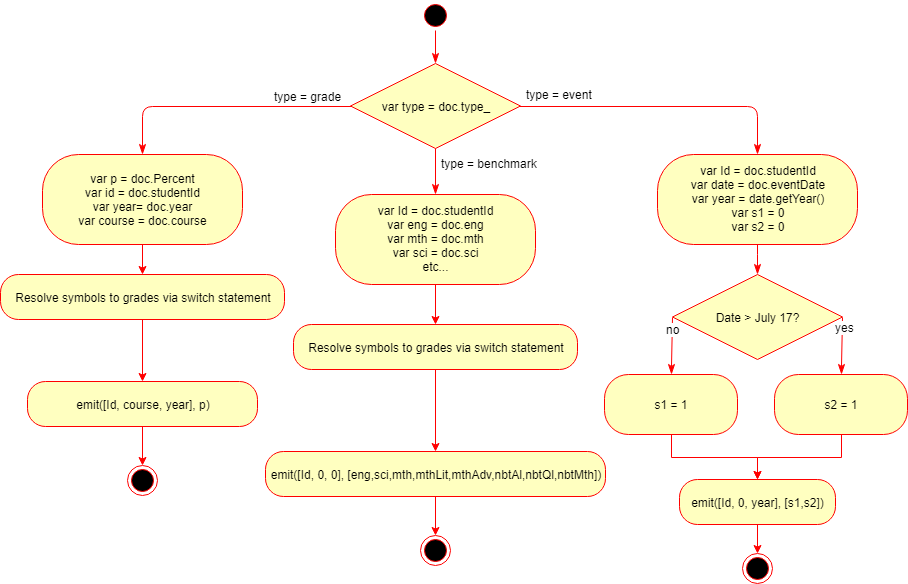
\includegraphics[scale=0.7]{./resources/figures/fig-mapfn-correlation-events.png}
    \end{mdframed}
    \caption[\textit{Map}-function: \texorpdfstring{(grades $\bowtie$ events) $\leftouterjoin$ admissions}{Lg}]{\textbf{Figure \ref{fig-mapfn-correlation-events}: \textit{Map}-function: \texorpdfstring{(grades $\bowtie$ events) $\leftouterjoin$ admissions}{Lg}}}
    \label{fig-mapfn-correlation-events}
\end{sidewaysfigure}


\subsection{Presentation}
A list function is implemented to retrieve the index with \mintinline{text}{reduce = true \& group = true} so that only reduced index output is retrieved, grouped by key.

Because the ranking of students for course grade and each benchmarking method is required, several ordered lists are kept in memory for the duration of time that a single course code is being processed (in this case CSC1015F). In other words, for each course code, and then for every result retrieved from the index, the student number from the row being processed is checked and compared to the student number from the previous row. If the current student number is not the same as the previous student number, then the current rows in memory are joined, and list of ranks for each course and benchmark are updated. It is necessary to process all index output for a particular course code before students can be ranked for a course (as well as ranked in terms of their benchmarks, when compared to other students who took that course).

As joins are performed, an object is kept in memory for each student, which keeps track of their course grade and scores for each benchmark. Once a single course’s results have been iterated over, ranking lists are created that comprise tuples of [StudentId, \%] and are ordered by the second index ($i = 1$). The object of students is updated to add a rankChange value for every benchmarking method compared to the course grade. This is worked out as $courseRank - benchmarkRank$.

Then, by iterating over the student object, it is possible to perform the summations stipulated in Equation \ref{eq:correlation}, and the correlation between change in class rank and events count is found (a separate correlation corresponding to each benchmark is obtained).

List function logic is represented as an activity diagram in Figure \ref{fig-listfn-correlation-events} and is configured to output a table of correlation coefficients for each benchmarking method as shown in Table \ref{tbl-correlation-events} (page \pageref{tbl-correlation-events}).

\begin{figure}[H]
    \centering
    \begin{mdframed}
        \centering
        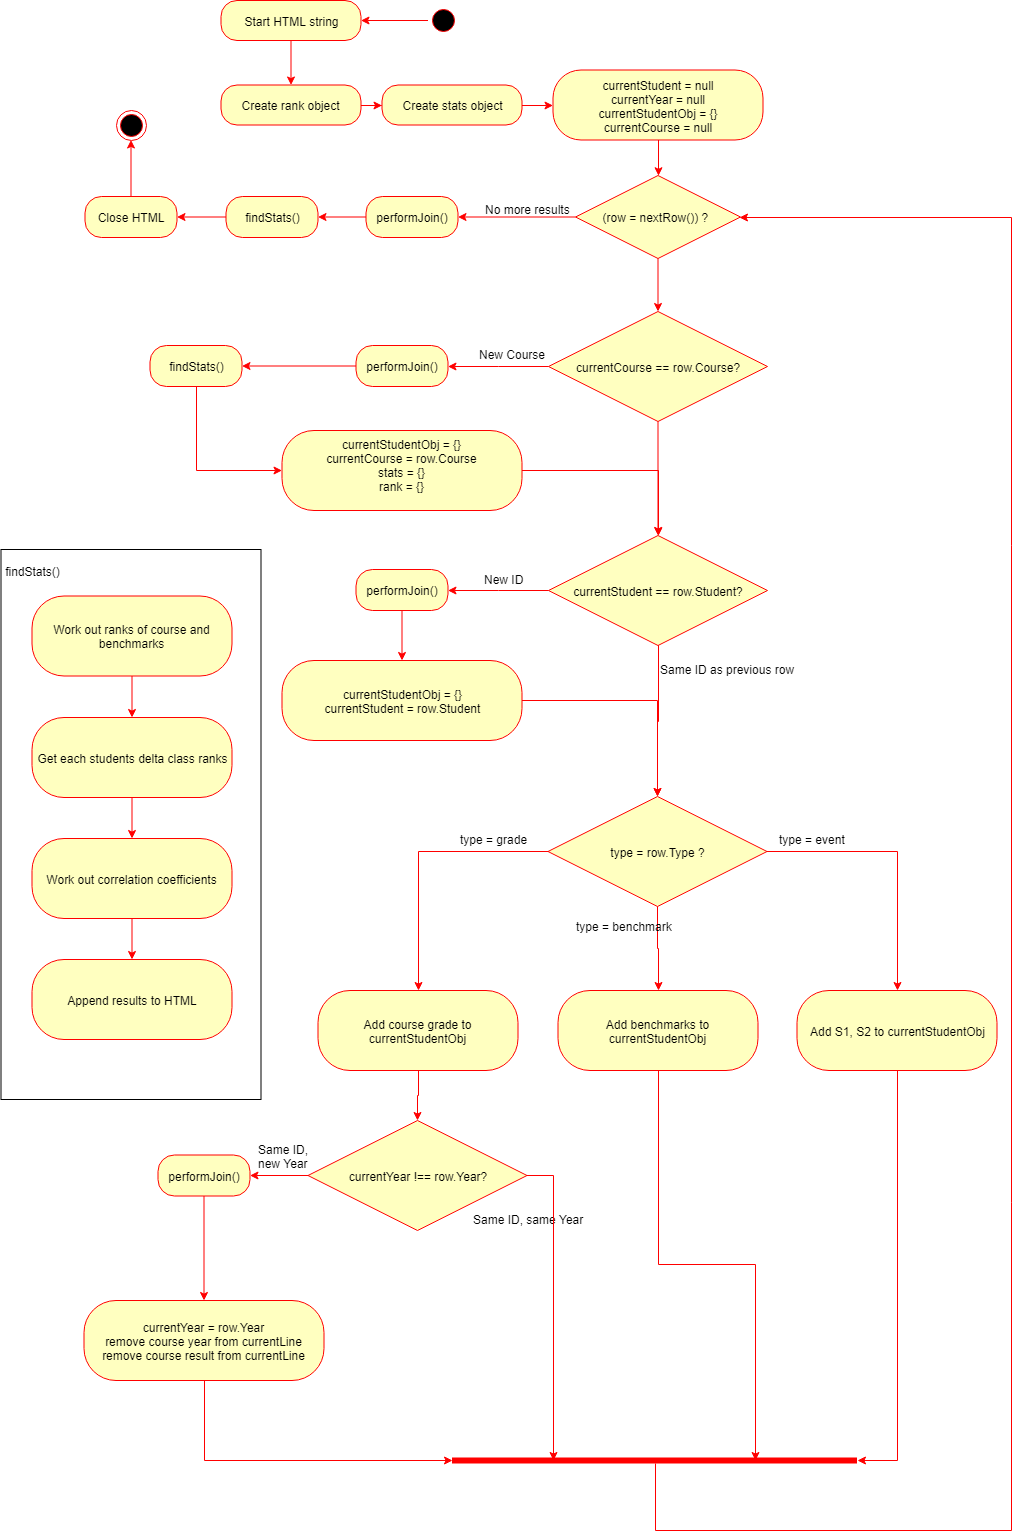
\includegraphics[scale=0.4]{./resources/figures/fig-listfn-correlation-events.png}
    \end{mdframed}
    \caption[\textit{List}-function: \texorpdfstring{(grades $\bowtie$ events) $\leftouterjoin$ admissions}{Lg}]{\textbf{\textit{List}-function: \texorpdfstring{(grades $\bowtie$ events) $\leftouterjoin$ admissions}{Lg}}}
    \label{fig-listfn-correlation-events}
\end{figure}


